\begin{tikzpicture}
    \begin{scope}[x={(0mm,300mm)},y={(0mm,199mm)},line width=1pt,cap=round]
        \node[anchor=south west,inner sep=0mm] at (0mm,0mm) {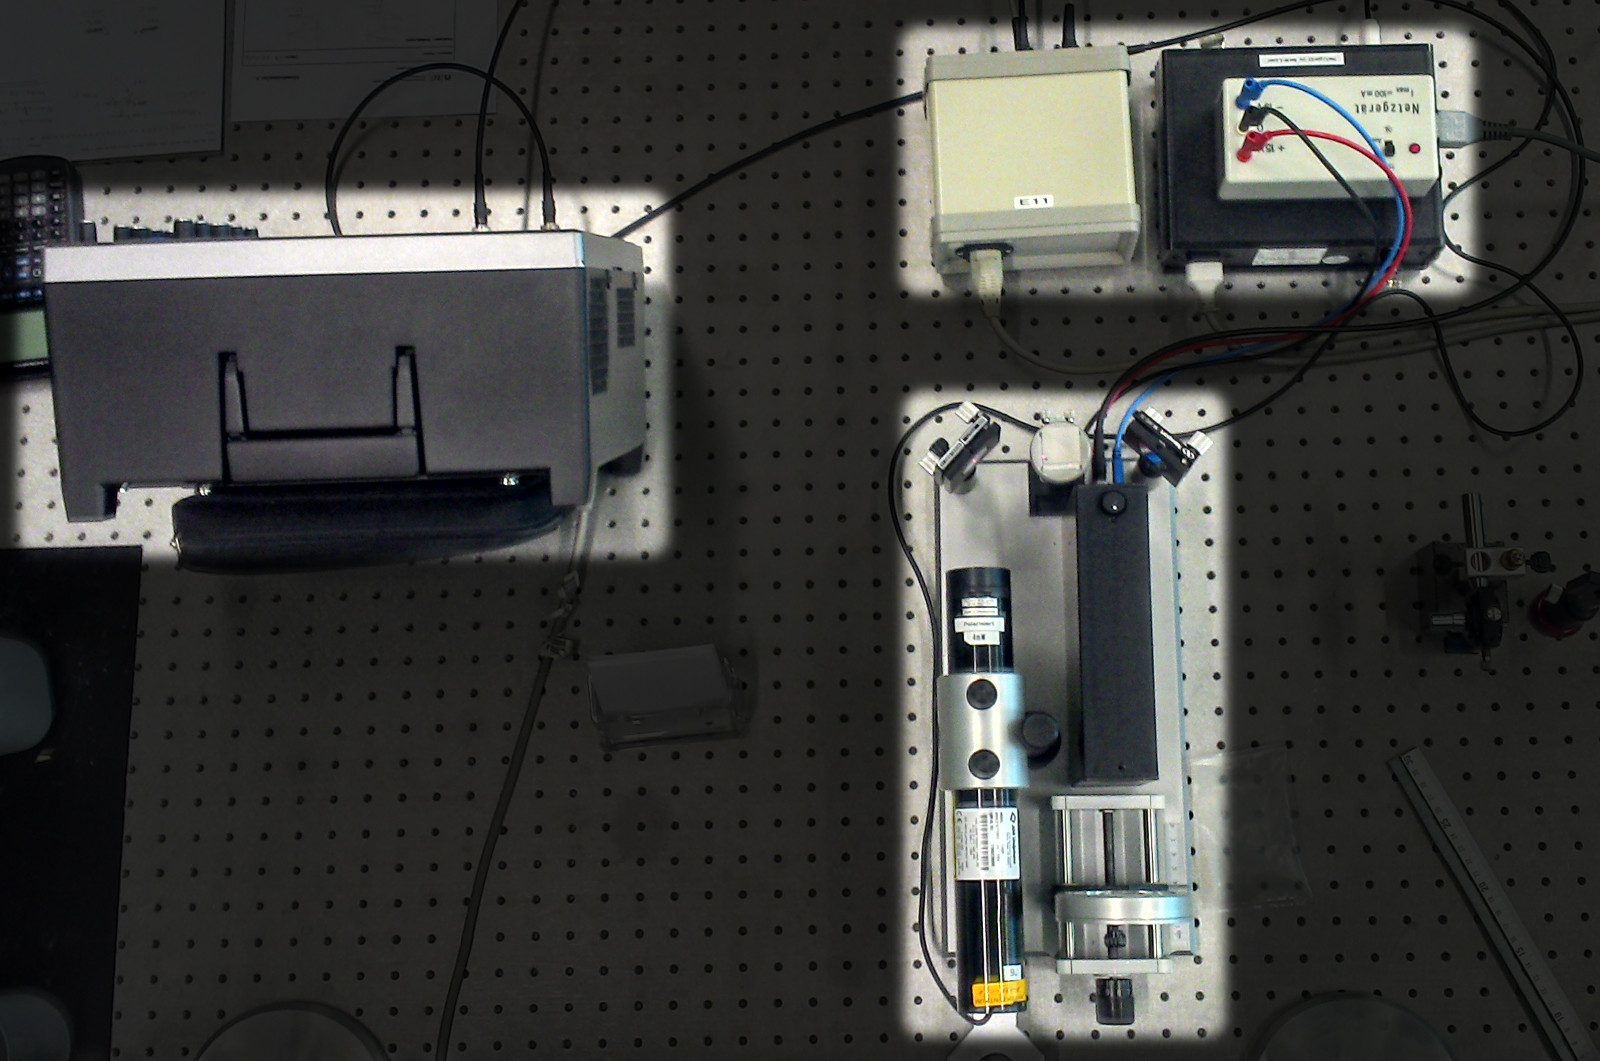
\includegraphics[width=300mm]{images/versuchsanordnung.jpeg}};

        % bounding box
        %\draw[green] (0mm,0mm) rectangle (300mm,199mm);

        \node[white] at (40mm,140mm) {\Large{Oszilloskop}};

        \node[white] at (160mm,50mm) {\Large{Laser}};

        \node[white] at (160mm,120mm) {\Large{Spiegel}};

        \draw[cyan] (225mm,30mm) -- (234mm,30mm);
        \node[white] at (245mm,30mm) {\Large{Linse $L_1$}};

        \draw[cyan] (210mm,80mm) -- (234mm,80mm);
        \node[white] at (250mm,80mm) {\Large{\parbox{30mm}{\raggedright Geh\"ause mit \\Photomultiplier,\\ Blende und Linse $L_2$}}};

        \draw[cyan] (225mm,120mm) -- (234mm,120mm);
        \node[white] at (245mm,120mm) {\Large{Spiegel}};

        \node[black] at (195mm,175mm) {\Large{Bandpassfilter}};

        \node[white] at (235mm,157.5mm) {\Large{Netzger\"ate}};
    \end{scope}
\end{tikzpicture}
